\input templates/header
\title[ASD - Introduzione]{\textbf{Algoritmi e Strutture Dati}\\[24pt]Introduzione}

\graphicspath{{figs/01/}}

\begin{document}

%-------------------------------------------------------------------------
\FrameTitle{}

%-------------------------------------------------------------------------
\FrameContent


%%%%%%%%%%%%%%%%%%%%%%%%%%%%%%%%%%%%%%%%%%%%%%%%%%%%%%%%%%%%%%%%%%%%%%%%%%
\section{Introduzione}

%-------------------------------------------------------------------------
%\begin{frame}[shrink=5]{Introduzione}
\begin{frame}{Introduzione}

\vspace{-9pt}
\begin{myboxtitle}[Problema computazionale]
Dati un dominio di input e un dominio di output, un \emph{\alert{problema computazionale}} 
è rappresentato dalla \alert{relazione matematica} che associa un elemento del dominio di output ad ogni elemento del dominio di input.
\end{myboxtitle}

\begin{myboxtitle}[Algoritmo]
Dato un problema computazionale, un \emph{\alert{algoritmo}}  è un procedimento 
\alert{effettivo}, 
espresso tramite un insieme di \alert{passi elementari ben specificati} 
in un sistema \alert{formale} di calcolo, che risolve il problema in tempo \alert{finito}.
\end{myboxtitle}

% \begin{myboxtitle}[Esempio classico, ma ingannevole...]
% \begin{columns}
% \begin{column}{0.48\textwidth}
% \begin{itemize}
% \item Input: \emph{ingredienti}
% \item Algoritmo: \emph{ricetta}
% \end{itemize}
% \end{column}
% \begin{column}{0.48\textwidth}
% \begin{itemize}
% \item Esecutore: \emph{cuoco}
% \item Output: \emph{piatto cucinato}
% \end{itemize}
% \end{column}
% \end{columns}
% \end{myboxtitle}
	
\end{frame}

%-------------------------------------------------------------------------
\begin{frame}{Algoritmi nella storia}
\BIL
\item Papiro di Rhind o di Ahmes (1850BC): algoritmo del contadino per la moltiplicazione
\item Algoritmi di tipo numerico furono studiati da matematici babilonesi ed indiani
\item Algoritmi in uso fino a tempi recenti furono studiati dai matematici greci più di 2000 anni fa
\begin{itemize}
\item Algoritmo di Euclide per il massimo comune divisore
\item Algoritmi geometrici (calcolo di tangenti, sezioni di angoli, ...)
\EIL
\end{itemize}

\begin{center}
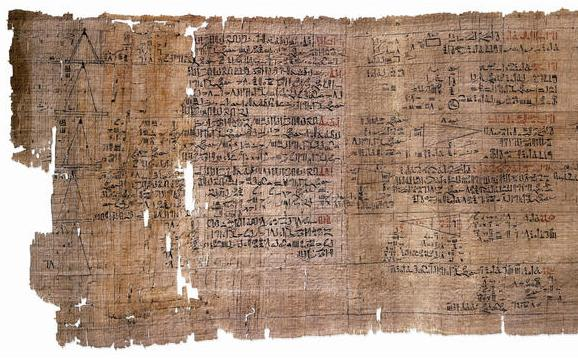
\includegraphics[width=4.5cm]{papyrus.jpg}
\end{center}
\tiny
\url{https://en.wikipedia.org/wiki/Rhind_Mathematical_Papyrus}
\end{frame}

%-------------------------------------------------------------------------
\begin{frame}[shrink=5]{Origine del nome}
	
\vspace{-12pt}
\begin{columns}[T]
\begin{column}{0.80\textwidth}	
\begin{myboxtitle}[\small Abu Abdullah Muhammad bin Musa \alert{al-Khwarizmi}]
\medskip
\begin{itemize}
\item E' stato un matematico, astronomo, astrologo e geografo 
\item Nato in Uzbekistan, ha lavorato a Baghdad
\item Dal suo nome: \alert{algoritmo}
\end{itemize}
\end{myboxtitle}
\end{column}
\begin{column}{0.18\textwidth}	
\begin{center}
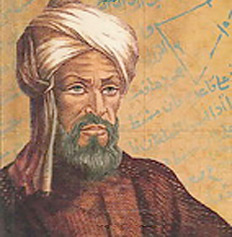
\includegraphics[width=2.3cm]{alkhavarizmi.jpg}
\end{center}
\end{column}
\end{columns}


\begin{overprint}
\onslide<1|handout:1>

\begin{columns}[T]
\column{0.80\textwidth}	

\begin{myboxtitle}[Algoritmi de numero indorum]
\begin{itemize}
\item Traduzione latina di un testo arabo ormai perso
\item Ha introdotto i numeri indiani (arabi) nel mondo occidentale
\item Dal numero arabico \alert{sifr} = 0: zephirum $\rightarrow$ zevero $\rightarrow$ zero, ma anche cifra
\end{itemize}
\end{myboxtitle}

\column{0.18\textwidth}	
\begin{center}

\includegraphics[width=2.3cm]{indorum.jpg}
\end{center}
\end{columns}

\onslide<2|handout:2>
\begin{columns}[T]
\column{0.80\textwidth}	
\begin{myboxtitle}[\small Al-Kitab al-muhtasar fi hisab \alert{al-gabr} wa-l-muqabala]
\begin{itemize}
\item La sua opera più famosa (820 d.C.)
\item Tradotta in latino con il titolo:\\ \emph{Liber algebrae et almucabala}
\item Dal suo titolo: \alert{algebra}
\end{itemize}
\end{myboxtitle}
\column{0.18\textwidth}	
\begin{center}

\includegraphics[width=2.3cm]{algebra.jpg}
\end{center}
\end{columns}
\end{overprint}


\end{frame}

\section{Problemi e algoritmi}

\subsection{Primi esempi}

%-------------------------------------------------------------------------
\begin{frame}{Problemi computazionali: esempi}

\vspace{-9pt}
\begin{myboxtitle}[Esempio: Minimo]
Il minimo di un insieme $S$ è l'elemento di $S$ che è minore o uguale ad ogni elemento di $S$.
\[
  \Min(S) = a \Leftrightarrow \exists a \in S: \forall b \in S : a \leq b
\]
\end{myboxtitle}

\begin{myboxtitle}[Esempio: Ricerca]
Sia $S=s_1, s_2, \ldots, s_n$ una sequenza di dati ordinati e distinti, i.e.  $s_1 < s_2 < \ldots < s_n$. 
Eseguire una ricerca della posizione di un dato $v$ in $S$ consiste nel restituire un indice $i$ tale che 
$1 \leq i \leq n$, se $v$ è presente nella posizione $i$, oppure $0$, se $v$ non è presente.
\[
 \mathit{lookup}(S, v) = \begin{cases}
  i & \exists i \in \{1, \mldots, n\}: S_i = v \\
  0 & \textrm{altrimenti}
  \end{cases}
\]
\end{myboxtitle}

\end{frame}

%-------------------------------------------------------------------------
\begin{frame}{Algoritmi: esempi}

\vspace{-9pt}
\begin{myboxtitle}[Algoritmo: Minimo]
Per trovare il minimo di un insieme, confronta ogni elemento con tutti gli
altri; l’elemento che è minore di tutti è il minimo.
\end{myboxtitle}


\begin{myboxtitle}[Algoritmo: Ricerca]
Per trovare un valore $v$ nella sequenza $S$, confronta $v$ con tutti gli elementi di $S$, 
in sequenza, e restituisci la posizione corrispondente; restituisci $0$ 
se nessuno degli elementi corrisponde.
\end{myboxtitle}

\end{frame}

\subsection{Pseudo-codice}

%-------------------------------------------------------------------------
\begin{frame}{Problemi}

Le descrizioni precedenti presentano diversi problemi:

\BIL
\item {\large\alert{Descrizione}}
\BI
\item Descritti in linguaggio naturale, imprecisi
\item Abbiamo bisogno di un linguaggio più formale
\EI
\item {\large\alert{Valutazione}}
\BI
\item Esistono algoritmi “migliori” di quelli proposti?
\item Dobbiamo definire il concetto di migliore
\EI
\EIL

\end{frame}

%-------------------------------------------------------------------------
\begin{frame}{Come descrivere un algoritmo}

\BIL
\item E' necessario utilizzare una descrizione il più possibile formale
\item Indipendente dal linguaggio: “\alert{Pseudo-codice}”
\item Particolare attenzione va dedicata al livello di dettaglio
\BI
\item Da una ricetta di canederli, leggo:\\
“... amalgamate il tutto e fate riposare un quarto d'ora...”
\item Cosa significa “amalgamare”? Cosa significa “far riposare”? 
\item E perché non c'è scritto più semplicemente “prepara i canederli”?
\EI
\EIL

\end{frame}

%-------------------------------------------------------------------------
\begin{frame}{Esempio: pseudo-codice}

\vspace{-18pt}
\small
\TwoCols{
\begin{Procedure}
\caption[A]{\INTEGER \MIN($\INTEGER[\,]\ S$,\ \INTEGER\ $n$)}
\For{$i = 1$ \TO $n$}
{
  $\BOOLEAN\ \mathit{isMin} = \TRUE$\;
  \For{$j = 1$ \TO $n$}{
    \If{$i \neq j$ \AND\ $S[j] < S[i]$}{
	  $\mathit{isMin} = \FALSE$\;
	}
  }
  \If{$\mathit{isMin}$}{ \Return $S[i]$\;}
}
\end{Procedure}
}
{
\begin{Procedure}
\caption[A]{\INTEGER \textsf{lookup}($\INTEGER[\,]\ S$,\ \INTEGER\ $n$, \INTEGER\ $v$)}
\For{$i = 1$ \TO $n$}
{
  \If{$S[i] \Eq v$}{ \Return $i$\;}
}
\Return $0$\;
\end{Procedure}
}

\begin{tikzpicture}[remember picture,overlay]
    \node[xshift=-4.0cm,yshift=-7.0cm] at (current page.north east){%
    \frame{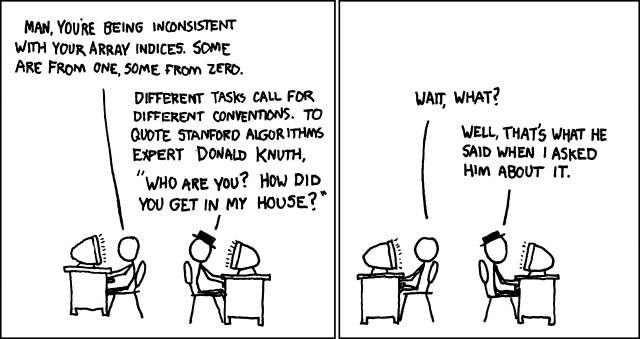
\includegraphics[width=7.5cm]{donald_knuth.png}}};
\end{tikzpicture}

\end{frame}

\begin{frame}{Pseudo-codice}

{\small 
\begin{columns}
\begin{column}{0.485\textwidth}
\begin{itemize}
\item $a = b$
\item $a \leftrightarrow b \ \equiv \ \mathit{tmp} = a; a = b; b = \mathit{tmp}$
\item $T[\,]\ A = \NEW\ T[1 \mldots n]$ \\
\item $T[\,][\,]\ B = \NEW\ T[1 \mldots n][1 \mldots m]$ \\
\item \INTEGER, \REAL, \BOOLEAN, \INTEGER
\item \AND, \OR, \NOT
\item $\Eq$, $\neq$, $\leq$, $\geq$
\item $+$, $-$, $\cdot$, $/$, $\lfloor x \rfloor$, $\lceil x \rceil$, $\log$, $x^2$, \mldots
\item $\textsf{iif}(\mathit{condizione}, v_1, v_2)$ 
\end{itemize}
\end{column}
\begin{column}{0.485\textwidth}
\begin{itemize}
\item \textbf{if} \emph{condizione} \textbf{then} istruzione
\item \textbf{if} \emph{condizione} \textbf{then} istruzione1 \textbf{else} istruzione2
\item \textbf{while} \emph{condizione} \textbf{do} istruzione
\item \textbf{foreach} \emph{elemento} $\in$ \emph{insieme} \textbf{do} istruzione
\item \textbf{return}
\item \% \emph{commento}
\end{itemize}
\end{column}
\end{columns}

}
\end{frame}

%-------------------------------------------------------------------------
\begin{frame}[shrink=10]{Pseudo-codice}

\small
\BI
\item \FOR \emph{indice} $=$ \emph{estremoInf} \textbf{to} \emph{estremoSup} \textbf{do} istruzione
\begin{minipage}{6cm}
\vspace{-9pt}
	\RestyleAlgo{plain}
	\begin{Procedure}	
	\INTEGER\ $\textit{indice} = \textit{estremoInf}$\;
	\While{$\textit{indice} \le \textit{estremoSup}$}
	{
	  $\textit{istruzione}$\;
	  $\textit{indice} = \textit{indice} + 1$\;
	}
	\end{Procedure}
	\RestyleAlgo{plain}
\vspace{-9pt}
\end{minipage}
\item \FOR \emph{indice} $=$ \emph{estremoSup} \textbf{downto} \emph{estremoInf} \textbf{do} istruzione
\begin{minipage}{6cm}
\vspace{-9pt}
	\RestyleAlgo{plain}
	\begin{Procedure}	
	\INTEGER\ $\textit{indice} = \textit{estremoSup}$\;
	\While{$\textit{indice} \ge \textit{estremoInf}$}
	{
	  $\textit{istruzione}$\;
	  $\textit{indice} = \textit{indice} - 1$\;
	}
	\end{Procedure}
	\RestyleAlgo{plain}
\vspace{-9pt}
\end{minipage}
\EI
\TwoCols{
\BI
\item $\Rettangolo\ r = \NEW\ \Rettangolo$\\
\item $r.\textit{altezza} = 10$\\
\item $\DELETE\ r$\\
\item $r = \Nil$\\
\EI
}
{\noindent
\begin{minipage}{4cm}
\begin{Procedure}
\caption{\Rettangolo}
\INTEGER \textit{lunghezza}\;
\INTEGER \textit{altezza}\;
\end{Procedure}
\end{minipage}
}
\end{frame}

\section{Valutazione}

%-------------------------------------------------------------------------
\begin{frame}{Come valutare l'algoritmo}

\vspace{-9pt}
\begin{myboxtitle}[Risolve il problema in modo \alert{efficiente}?]
\BIL
\item Dobbiamo stabilire come valutare se un programma è efficiente
\item Alcuni problemi non possono essere risolti in modo efficiente
\item Esistono soluzioni “ottime”: non è possibile essere più efficienti
\EIL
\end{myboxtitle}

\begin{myboxtitle}[Risolve il problema in modo \alert{corretto}?]
\BIL
\item  Dimostrazione matematica, descrizione “informale”
\item Nota: Alcuni problemi non possono essere risolti
\item Nota: Alcuni problemi vengono risolti in modo approssimato
\EIL
\end{myboxtitle}

\end{frame}

\subsection{Efficienza}

%-------------------------------------------------------------------------
\begin{frame}[shrink=10]{Charles Babbage}

\vspace{-9pt}
\begin{myboxtitle}[Passages from the Life of a Philosopher, Charles Babbage, 1864]
As soon as an Analytical Engine exists, it will necessarily guide the future
course of the science. Whenever any result is sought by its aid, the question
will then arise --- \alert{By what course of calculation can these results be arrived at
by the machine in the shortest time?}
\end{myboxtitle}

\vspace{-12pt}
\TwoCols{
\begin{center}
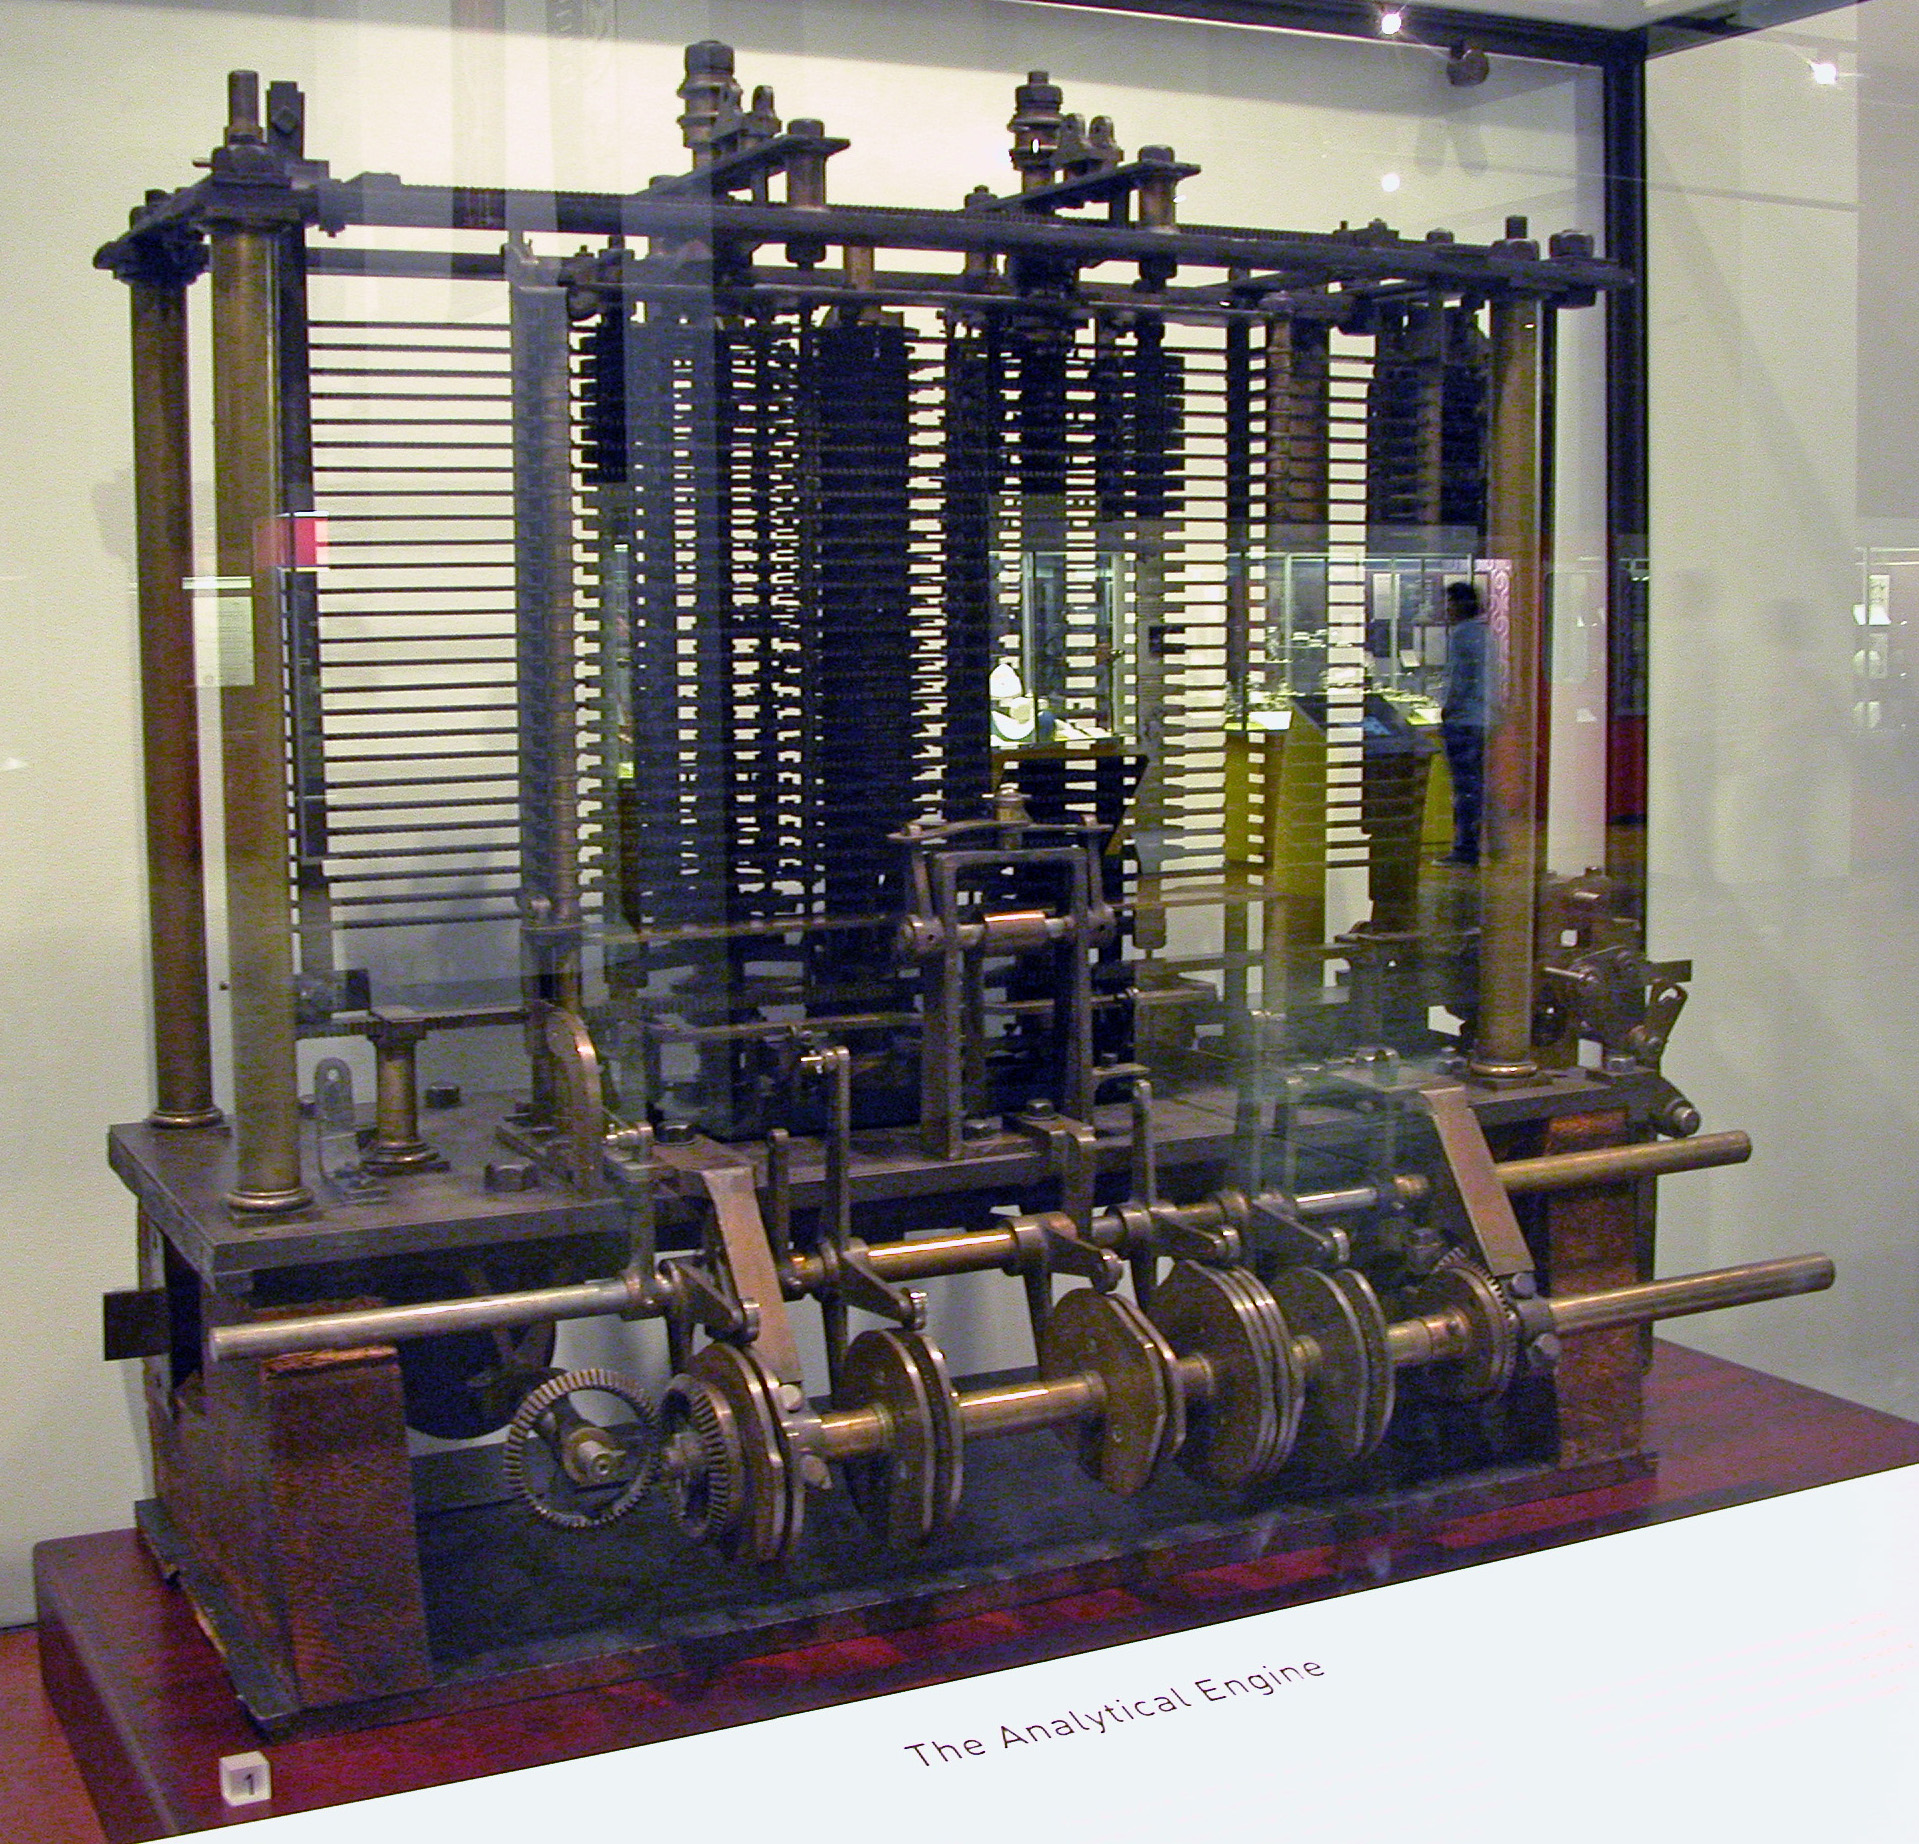
\includegraphics[width=3.75cm]{analytical.jpg}

\small{Modello della macchina analitica, Museo di Londra, foto Bruno Barral}
\end{center}
}{
\begin{center}
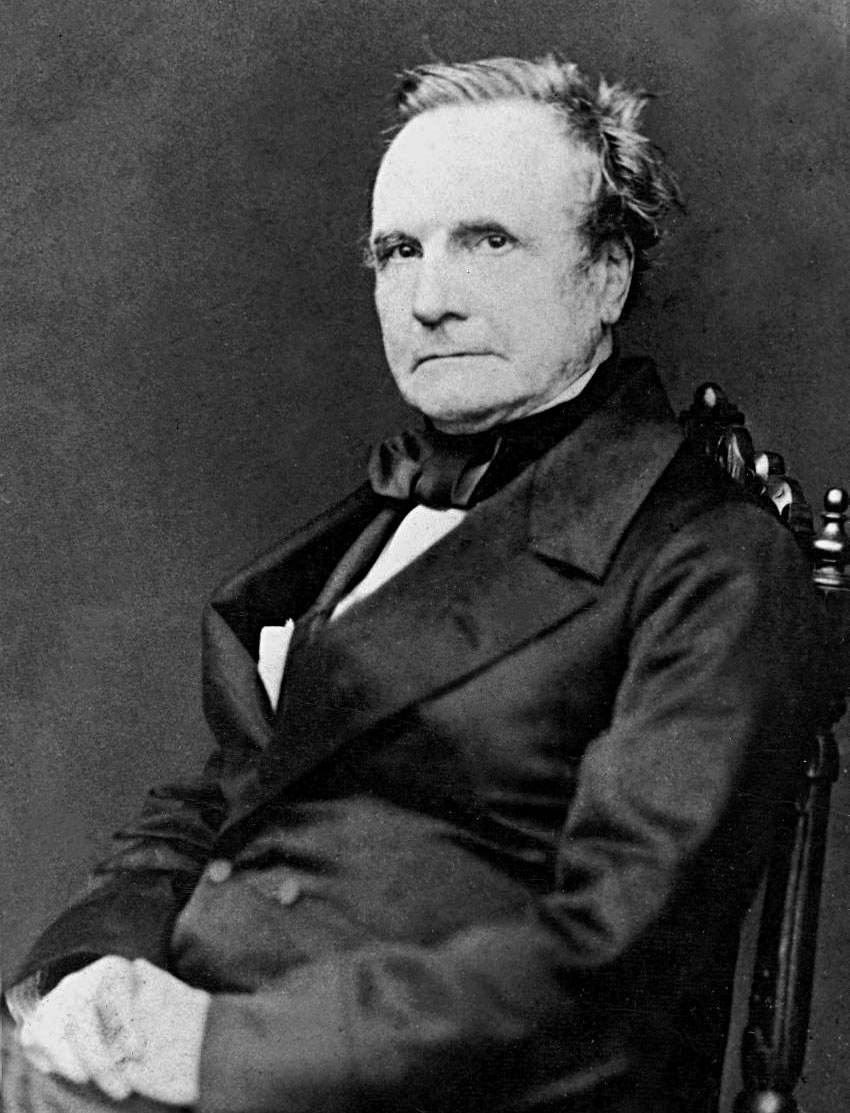
\includegraphics[width=3cm]{babbage.jpg}

\small{Charles Babbage, 1860}
\end{center}
}

\end{frame}

%-------------------------------------------------------------------------
\begin{frame}{Valutazione algoritmi -- Efficienza}
	
\vspace{-9pt}
\begin{myboxtitle}[Complessità di un algoritmo]
Analisi delle \alert{risorse} impiegate da un algoritmo per risolvere un problema, in
funzione della \alert{dimensione} e dalla \alert{tipologia} dell'input
\end{myboxtitle}

\medskip

\begin{myboxtitle}[Risorse]
\begin{itemize}
\item \alert{Tempo}: tempo impiegato per completare l'algoritmo
\begin{itemize}
	\item Misurato con il cronometro?
	\item Misurato contando il numero di operazioni rilevanti?
	\item Misurato contando il numero di operazioni elementari?
\end{itemize}
\item \alert{Spazio}: quantità di memoria utilizzata
\item \alert{Banda}: quantità di bit spediti (algoritmi distribuiti)
\end{itemize}

\end{myboxtitle}

\end{frame}

%-------------------------------------------------------------------------
\begin{frame}{Definizione di tempo}

\vspace{-9pt}
\begin{myboxtitle}[Tempo $\equiv$ wall-clock time]
Il tempo effettivamente impiegato per eseguire un algoritmo
\end{myboxtitle}


\begin{mybox}
Dipende da troppi parametri:
\BI
\item bravura del programmatore
\item linguaggio di programmazione utilizzato
\item codice generato dal compilatore
\item processore, memoria (cache, primaria, secondaria)
\item sistema operativo, processi attualmente in esecuzione
\EI
\end{mybox}

\begin{mybox}
\alert{Dobbiamo considerare una rappresentazione più astratta!}
\end{mybox}

\end{frame}

%-------------------------------------------------------------------------
\begin{frame}{Definizione di tempo -- A grandi linee}

\vspace{-9pt}
\begin{myboxtitle}[Tempo $\equiv$ n. operazioni rilevanti]
Numero di operazioni "rilevanti", ovvero il numero di operazioni che caratterizzano lo scopo dell'algoritmo.
\end{myboxtitle}

\begin{myboxtitle}[Esempio]
\BIL
\item Nel caso del minimo, numero di confronti \texttt{<}
\item Nel caso della ricerca, numero di confronti \texttt{==}
\EIL
\end{myboxtitle}

\begin{mybox}
\alert{Proviamo!}
\end{mybox}


\end{frame}


%-------------------------------------------------------------------------
\begin{frame}[shrink=10]{Valutazione algoritmi -- Minimo}

\vspace{-9pt}
\begin{mybox}
Contiamo il numero di confronti per il problema del \alert{minimo}
\end{mybox}

\TwoCols{
\begin{Procedure}
\caption[A]{\INTEGER \MIN($\INTEGER[\,]\ S$,\ \INTEGER\ $n$)}
\For{$i = 1$ \TO $n$}
{
  $\BOOLEAN\ \mathit{isMin} = \TRUE$\;
  \For{$j = 1$ \TO $n$}{
    \If{$i \neq j$ \AND\ $S[j] < S[i]$}{
	  $\mathit{isMin} = \FALSE$\;
	}
  }
  \If{$\mathit{isMin}$}{ \Return $S[i]$\;}
}
\end{Procedure}
}{
\pause
\begin{mybox}
Algoritmo “naïf”: \alert{$n^2-n$} 
\end{mybox}

\begin{mybox}
Si può fare meglio di così?
\end{mybox}

}

\end{frame}

\begin{frame}[t]{Valutazione algoritmi -- Un algoritmo migliore}

\vspace{-9pt}
\begin{mybox}
Contiamo il numero di confronti per il problema del \alert{minimo}
\end{mybox}

\TwoColsCustom{0.55}{0.43}{
\begin{Procedure}
\caption[A]{\INTEGER \MIN($\INTEGER[\,]\ S$,\ \INTEGER\ $n$)}
\Comment{Partial minimum}
\INTEGER $\Min = S[1]$\;
\For{$i = 2$ \TO $n$}
{
  
  \If{$S[i] < \Min$}{
     \Comment{Update partial minimum}
     $\Min = S[i]$}
  }
\Return $\Min$
\end{Procedure}
}{
\pause
\begin{mybox}
Algoritmo “naïf”: \alert{$n^2-n$} 
\end{mybox}
\begin{mybox}
Algoritmo efficiente: \alert{$n-1$} 
\end{mybox}

}
\end{frame}

\begin{frame}[shrink=10]{Valutazione algoritmi -- Ricerca}

\vspace{-9pt}
\begin{mybox}
Contiamo il numero di confronti per il problema della \alert{ricerca}
\end{mybox}


\TwoCols{
\begin{Procedure}
\caption[A]{\INTEGER \textsf{lookup}($\INTEGER[\,]\ S$,\ \INTEGER\ $n$, \INTEGER\ $v$)}
\For{$i = 1$ \TO $n$}
{
  \If{$S[i] \Eq v$}{ \Return $i$\;}
}
\Return $0$\;
\end{Procedure}
}{
\begin{mybox}
Algoritmo “naïf”: \alert{$n$} 
\end{mybox}

\begin{mybox}
Si può fare meglio di così?
\end{mybox}
}
\end{frame}

\begin{frame}{Valutazione algoritmi -- Un algoritmo migliore}

\vspace{-9pt}
\begin{myboxtitle}[Una soluzione più efficiente]
Analizzo l'elemento centrale (indice $m$) del sottovettore considerato:

\BIL
  \item Se $A[m]=v$, ho trovato il valore cercato
  \item Se $v<A[m]$, cerco nella “metà di sinistra”
  \item Se $A[m]<v$, cerco nella “metà di destra”
\EIL
\end{myboxtitle}

\vspace{-24pt}
\begin{overprint}
\onslide<1|handout:1>\centering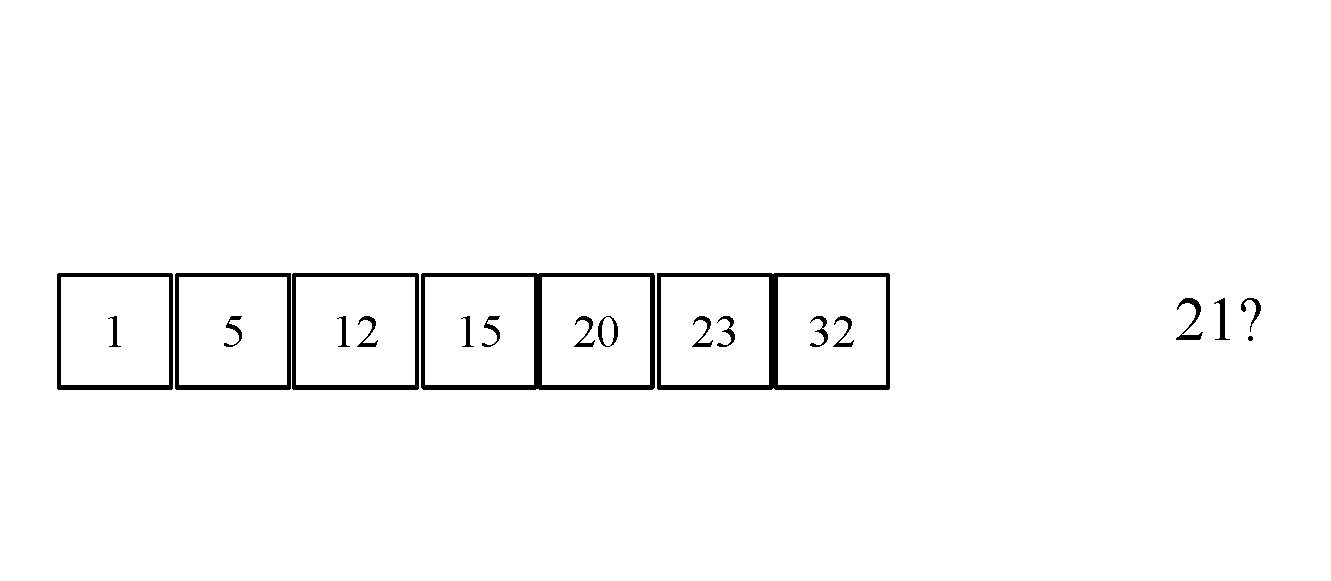
\includegraphics[width=10cm,page=1]{binarysearch.pdf}
\onslide<2|handout:2>\centering\includegraphics[width=10cm,page=2]{binarysearch.pdf}
\onslide<3|handout:3>\centering\includegraphics[width=10cm,page=3]{binarysearch.pdf}
\onslide<4|handout:4>\centering\includegraphics[width=10cm,page=4]{binarysearch.pdf}
\onslide<5|handout:5>\centering\includegraphics[width=10cm,page=5]{binarysearch.pdf}
\onslide<6|handout:6>\centering\includegraphics[width=10cm,page=6]{binarysearch.pdf}
\onslide<7|handout:7>\centering\includegraphics[width=10cm,page=7]{binarysearch.pdf}
\onslide<8|handout:8>\centering\includegraphics[width=10cm,page=8]{binarysearch.pdf}
\end{overprint}


\end{frame}

\begin{frame}[shrink=10]{Valutazione algoritmi -- Un algoritmo migliore}

\vspace{-9pt}
\begin{mybox}
Contiamo il numero di confronti per il problema della \alert{ricerca}
\end{mybox}

\vspace{-12pt}
\TwoColsCustom{0.57}{0.40}{
\begin{Procedure}
\caption[A]{\INTEGER\ \binarysearch($\INTEGER[\,]\ S$, $\INTEGER\ v$, \INTEGER $i$, \INTEGER $j$)}

\eIf{$i>j$}{
  \Return $0$\;
}
{
  \INTEGER $m = \lfloor (i+j)/2 \rfloor$\;
  \uIf{$S[m] \Eq v$}{ 
    \Return $m$\; 
  }
  \uElseIf{$S[m] < v$}{
    \Return $\binarysearch(S, v, m+1, j)$\;
  }
  \Else {
    \Return $\binarysearch(S, v, i, m-1)$\;  
  }
}
\end{Procedure}
}{
\pause
\begin{mybox}
Algoritmo “naïf”: \alert{$n$} 
\end{mybox}
\begin{mybox}
Algoritmo efficiente:\newline \alert{$\lceil \log n \rceil$} 
\end{mybox}
}

\end{frame}



\subsection{Correttezza}

\begin{frame}{Valutazione algoritmi -- Correttezza}

\vspace{-9pt}
\begin{myboxtitle}[Invariante]
Condizione sempre vera in un certo punto del programma
\end{myboxtitle}

\begin{myboxtitle}[Invariante di ciclo]
\begin{itemize}
\item Una condizione sempre vera all'inizio dell'iterazione di un ciclo
\item Cosa si intende per "inizio dell'iterazione"?
\end{itemize}
\end{myboxtitle}

\begin{myboxtitle}[Invariante di classe]
\begin{itemize}
\item Una condizione sempre vera al termine dell'esecuzione di un metodo della classe
\end{itemize}
\end{myboxtitle}

\end{frame}

\begin{frame}{Valutazione algoritmi -- Correttezza}

\vspace{-9pt}
\begin{mybox}
Il concetto di \alert{invariante di ciclo} ci aiuta a dimostrare la correttezza di un \alert{algoritmo iterativo}.
\end{mybox}

\begin{itemize}
\item \alert{Inizializzazione} (caso base): 

La condizione è vera alla prima iterazione di un ciclo

\item \alert{Conservazione} (passo induttivo):

Se la condizione è vera prima di un'iterazione del ciclo, allora rimane vera al termine (quindi prima della successiva iterazione)

\item \alert{Conclusione}:

Quando il ciclo termina, l'invariante deve rappresentare la “correttezza” dell'algoritmo

\end{itemize}

\end{frame}

\begin{frame}{Valutazione algoritmi -- Correttezza}
	
\begin{mybox}
All'inizio di ogni iterazione del ciclo \textbf{for}, la variabile $\Min$ contiene il minimo parziale degli 
elementi $S[1 \ldots i-1]$.
\end{mybox}

\TwoCols{
\begin{Procedure}
\caption[A]{\INTEGER \MIN($\INTEGER[\,]\ S$,\ \INTEGER\ $n$)}
\INTEGER $\Min = S[1]$\;
\For{$i = 2$ \TO $n$}
{
  \If{$S[i] < \Min$}{ $\Min = S[i]$}
}
\Return $\Min$
\end{Procedure}
}{
\begin{mybox}
Inizializzazione
\end{mybox}
\begin{mybox}
Conservazione
\end{mybox}
\begin{mybox}
Conclusione
\end{mybox}
}
\end{frame}



\begin{frame}[shrink=7]{Valutazione algoritmi -- Correttezza}

\vspace{-9pt}
\begin{mybox}
La dimostrazione per induzione è utile anche con gli algoritmi ricorsivi
\end{mybox}

\vspace{-12pt}
\TwoColsCustom{0.59}{0.38}{
\begin{Procedure}
\caption[A]{\INTEGER\ \binarysearch($\INTEGER[\,]\ A$, \INTEGER $v$, \INTEGER $i$, \INTEGER $j$)}

\uIf{$i>j$}{
  \Return $0$\;
}
\Else
{
  \INTEGER $m = \lfloor (i+j)/2 \rfloor$\;
  \uIf{$A[m] \Eq v$}{ 
    \Return $m$\; 
  }
  \uElseIf{$A[m] < v$}{
    \Return $\binarysearch(A, v, m+1, j)$\;
  }
  \Else {
    \Return $\binarysearch(A, v, i, m-1)$\;  
  }
}
\end{Procedure}
}{
\begin{mybox}
Per induzione sulla\\
dimensione $n$ dell'input
\end{mybox}
\BIL
\item \alert{Caso base}:\\ $n=0$ ($i>j$)
\item \alert{Ipotesi induttiva}:\\ vero per tutti gli $n'<n$
\item \alert{Passo induttivo}:\\
  dimostrare che è vero per $n$
\EIL
}

\end{frame}


\section{Conclusioni}

\begin{frame}{Altre proprietà}

Semplicità, modularità, manutenibilità, espandibilità, robustezza, \ldots
\begin{itemize}
\item Secondari in un corso di algoritmi e strutture dati
\item Fondamentali per un corso di ingegneria del software
\end{itemize}

\medskip
\begin{myboxtitle}[Commento]
Alcune proprietà hanno un costo aggiuntivo in termini di prestazioni
\begin{itemize}
\item \makebox[3cm][l]{Codice modulare} $\rightarrow$ costo gestione chiamate
\item \makebox[3cm][l]{Java bytecode} $\rightarrow$ costo interpretazione
\end{itemize}
\begin{quote}
Progettare algoritmi efficienti è un prerequisito per poter pagare questo costo
\end{quote}
\end{myboxtitle}	
	
\end{frame}

\begin{OnlySlides}{Binary search, in pillole}
\begin{center}
    \IG{1.0}{binary-search.png}
\end{center}
\end{OnlySlides}


\end{document}





